\documentclass[10pt]{article}
\usepackage[margin=0.75in]{geometry}
\usepackage{url}
\usepackage{graphicx}
\usepackage{array}
\usepackage{tabularx}
\usepackage{float}
\usepackage{xcolor}
\usepackage{tikz}
\usetikzlibrary{arrows.meta,positioning,shapes.geometric}
\graphicspath{{../results/figures/}}
\newcolumntype{Y}{>{\raggedright\arraybackslash}X}
\tikzset{
  copperpicture/.style={node distance=8mm and 10mm},
  copperbox/.style={draw, rounded corners=1.5pt, align=center, font=\footnotesize, inner sep=4pt, minimum height=8mm, text width=24mm, fill=gray!5},
  copperwide/.style={copperbox, text width=30mm},
  coppergate/.style={diamond, draw, aspect=2, align=center, font=\footnotesize, inner sep=2pt, text width=20mm, fill=orange!12},
  copperblock/.style={draw, dashed, rounded corners=1.5pt, align=center, font=\footnotesize, inner sep=4pt, text width=26mm, fill=red!6},
  copperok/.style={copperbox, fill=green!8},
  copperarrow/.style={-{Latex[length=2mm]}, thick},
  copperclear/.style={-{Latex[length=2mm]}, thick, dashed}
}

\title{COPPER: Committed Pointer-Provenance Prefetching}
\author{Anonymous Artifact Submission}
\date{}

\begin{document}
\maketitle

\begin{abstract}
Data-derived prefetchers can reduce pointer-chasing latency, but they can also turn address-shaped data into prefetch authority before the program has proved that the data is a pointer. COPPER addresses that authority problem with committed pointer-provenance prefetching: it records pointer-source evidence only after architectural commit, invalidates stale or mismatched evidence, and gates later data-derived prefetch issue on that committed evidence. This submission frames COPPER as an evidence-bounded reproducible hardware mechanism study evaluated with CI-proven RTL simulation, raw gem5 full-system provenance where retained, validated imported gem5 ARM-system summaries where PASS, independent simulator evidence, accepted-core-wrapper/PicoRV32 tiny-SoC full-core FPGA mapped PPA, and tool-estimated/proxy power. The supported claim is auditable at the stated evidence levels. It does not claim state-of-the-art performance, production readiness, a complete clone-local gem5 campaign, production ARM/OoO integration, production-core mapped timing, measured silicon power efficiency, ASIC signoff, foundry signoff, or silicon signoff.
\end{abstract}

\section{Introduction}
Pointer-heavy programs expose memory latency that ordinary address-stream prefetchers can miss. Data-derived prefetching can help by following loaded values, but the same behavior is risky when a value merely resembles an address. COPPER changes the authority rule: a prefetch candidate needs committed pointer-source evidence before issue. The mechanism is meant to filter unsafe or stale candidates while preserving the useful subset of pointer-derived prefetches.

This paper makes an evidence-bounded contribution. COPPER is evaluated as a reproducible hardware mechanism, not as a silicon product or a production processor feature. The evidence consists of executable model checks, deterministic cycle-model and core-integrated rows, source-backed independent simulator rows, validated gem5 ARM-system summaries and retained raw gem5 provenance where available, CI-proven RTL unit simulation, accepted-core-wrapper/PicoRV32 tiny-SoC full-core mapped FPGA PPA, FPGA tool-estimated power, and proxy energy. The artifact keeps these evidence levels separate and keeps negative rows visible.

This paper does not claim silicon-proven status, ASIC/foundry signoff, measured silicon power, production ARM/OoO/TLB/cache/coherence integration, state-of-the-art silicon efficiency, universal speedup, production readiness, or full silicon PPA. The claim ledger and audits are part of the submission: if the paper drifts into unsupported language, the artifact should fail.

\section{Motivation}
\begin{figure}[H]
\centering
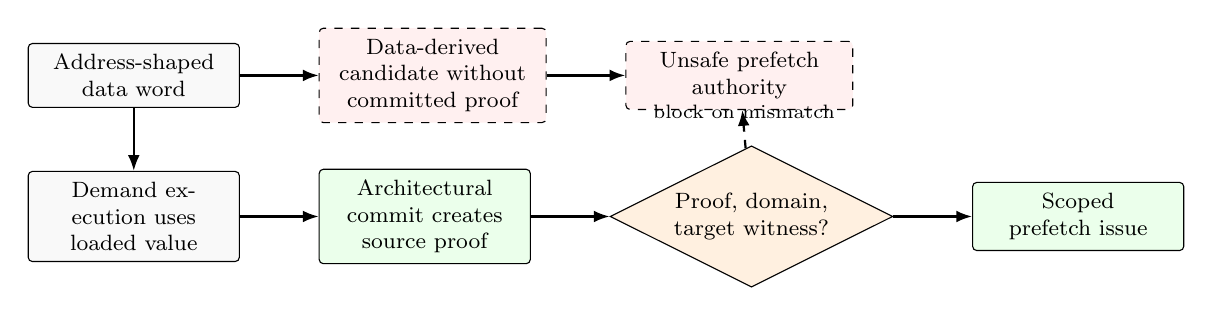
\begin{tikzpicture}[copperpicture]
\node[copperbox] (data) {Address-shaped data word};
\node[copperblock, right=of data] (unsafe) {Data-derived candidate without committed proof};
\node[copperblock, right=of unsafe] (badissue) {Unsafe prefetch authority};
\node[copperbox, below=of data] (demand) {Demand execution uses loaded value};
\node[copperok, right=of demand] (commit) {Architectural commit creates source proof};
\node[coppergate, right=of commit] (gate) {Proof, domain, target witness?};
\node[copperok, right=of gate] (safeissue) {Scoped prefetch issue};
\draw[copperarrow] (data) -- (unsafe);
\draw[copperarrow] (unsafe) -- (badissue);
\draw[copperarrow] (data) -- (demand);
\draw[copperarrow] (demand) -- (commit);
\draw[copperarrow] (commit) -- (gate);
\draw[copperarrow] (gate) -- (safeissue);
\draw[copperclear] (gate) -- node[above, font=\scriptsize] {block on mismatch} (badissue);
\end{tikzpicture}
\caption{Pointer-chasing authority problem and COPPER's evidence-gated alternative. A data value alone is not enough authority; issue is allowed only after committed source proof and target checks agree.}
\label{fig:motivation}
\end{figure}

The motivating failure mode is not ordinary speculation alone. It is that a prefetcher may treat address-shaped data as authority, a concern sharpened by recent data-memory-dependent prefetcher attacks \cite{augury,gofetch}. COPPER instead treats committed pointer use as authority.

\section{Background And Related Work}
Prior work covers next-line, stream, stride, indirect, pointer-chase, runahead, helper-thread, and dependence-guided prefetching \cite{jouppi1990improving,chen1995effective,baer1991effective,roth1998dependence,srinath2007feedback}, as well as metadata and capability mechanisms \cite{cheri}. COPPER's distinction is narrower: committed source-word proof gates data-derived prefetch issue. The repository matrix records what COPPER does not claim.

Recent DMP attack and vendor material make the authority problem concrete: a data-dependent prefetcher may examine memory data and create cache-visible effects from the derived target \cite{augury,gofetch,intelDDP}. Software and OS defenses such as memory representation transformation or scheduler-managed prefetcher disablement address adjacent deployment points \cite{splittingsecrets,prefence}. Shadow-structure speculation defenses isolate speculative side effects until commit; COPPER instead scopes the authority of a non-speculative data-derived prefetch path \cite{safespec}.

\begin{table}[H]
\centering
\caption{Related Work Positioning}
\label{tab:related-positioning}
\begin{tabularx}{\linewidth}{YYYY}
\hline
Adjacent area & Typical focus & COPPER distinction & Claim boundary \\
\hline
Data-memory-dependent attacks & Show that data values can trigger observable prefetch behavior & Replaces address-shapedness with committed source-word authority & Attack surface is the DMP authority path, not all channels \\
Pointer-chase and indirect prefetching & Expose irregular memory parallelism from pointer-like streams & Allows issue only after the source word has committed-use proof & Does not claim pointer prefetching itself \\
Confidence and usefulness filters & Suppress candidates predicted to be inaccurate or wasteful & Blocks candidates that lack architectural authority even when they look useful & Performance regressions remain visible per row \\
Capability, tag, and taint mechanisms & Track architectural permissions, memory safety, or information flow & Tracks a small positive proof for microarchitectural DMP dereference permission & Does not replace architectural memory-safety mechanisms \\
Software or OS DMP defenses & Transform data or disable prefetching in sensitive regions & Keeps the hardware gate active at source-word granularity & Does not make compiler or OS policies obsolete \\
Runahead and translation aids & Expose misses or accelerate address translation & Recursive and cross-page issue stay bound to source proof and target witnesses & Not a general runahead or translation accelerator \\
\hline
\end{tabularx}
\end{table}

\section{Threat Model And Security Contract}
COPPER targets data-memory-dependent prefetch issue where address-shaped data, stale pointer values, or mismatched address-space state could otherwise create cache-visible prefetch activity before the program has committed a pointer use. The adversary model is scoped to the prefetch authority decision: an adversary may influence data values and observe cache or memory-system side effects, while ordinary demand accesses, branch predictor channels, non-DMP microarchitectural channels, and full operating-system isolation policy are outside this mechanism-level contract.

The security contract is intentionally small: a data-derived candidate may issue only when committed source proof exists, the source proof remains clean and current, the target authority check succeeds, and the candidate is still bound to the same relevant context. Table~\ref{tab:security-contract} maps the main reviewer attack surfaces to the local evidence that exercises the rule.

\begin{table}[H]
\centering
\caption{Security Contract And Evidence}
\label{tab:security-contract}
\begin{tabularx}{\linewidth}{YYY}
\hline
Reviewer concern & COPPER contract response & Evidence anchor \\
\hline
Address-shaped data at rest & No committed source proof, so the issue gate blocks data-only candidates & \path{COPPER_SECURITY_COVERAGE_MATRIX.md}; \path{model_tests.csv}; \path{rtl_simulation.csv} \\
Stale source after write or coherence activity & Source proof is cleared or fails epoch/value freshness checks before issue & \path{COPPER_AUTHORITY_REGRESSION_SUMMARY.md}; \path{COPPER_CEPF_LINE_E2E_SVA_SUMMARY.md} \\
Recursive or cross-page target issue & Target-line witness and translation/permission checks are required before issue & \path{COPPER_CTLW_FULL_AUTHORITY_E2E_SUMMARY.md}; \path{COPPER_CAVI_AUTHORITY_ISSUE_GATE_RTL_SUMMARY.md} \\
Context remap, permission, or revocation & Domain and revocation checks are part of the authority path, and missing evidence blocks the candidate & \path{COPPER_TLB_COHERENCE_AUTHORITY_FILTER_RTL_SUMMARY.md}; \path{COPPER_SARI_CLPD_CTLW_AUTHORITY_E2E_SUMMARY.md} \\
Broader microarchitectural isolation & Out of scope for this artifact; stronger production and silicon claims remain blocked by the claim ledger & \path{COPPER_CLAIM_LEDGER.md}; \path{stronger_claim_audit.csv} \\
\hline
\end{tabularx}
\end{table}

\section{COPPER Design}
\begin{figure}[H]
\centering
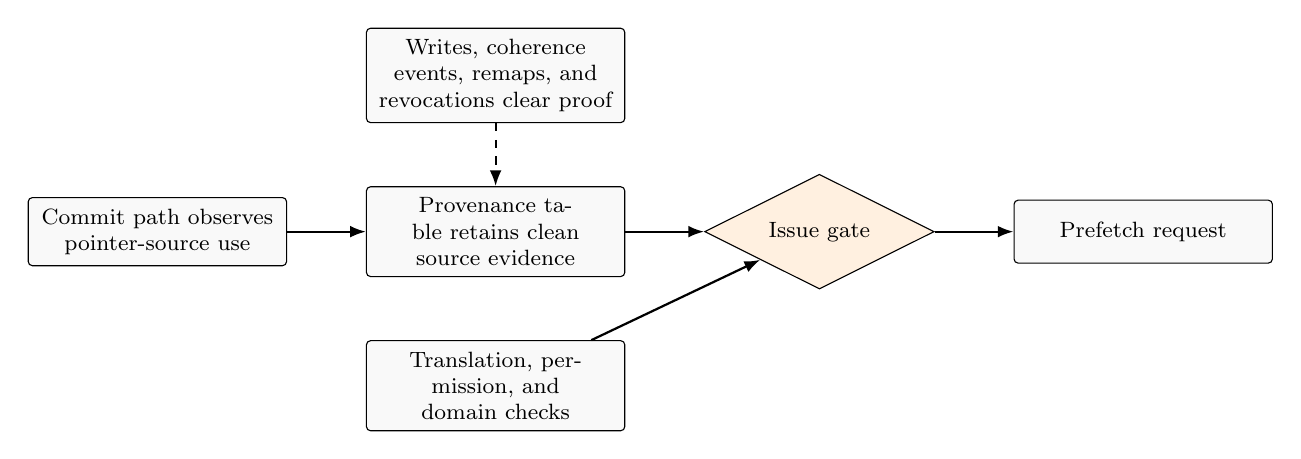
\begin{tikzpicture}[copperpicture]
\node[copperwide] (commit) {Commit path observes pointer-source use};
\node[copperwide, right=of commit] (proof) {Provenance table retains clean source evidence};
\node[coppergate, right=of proof] (issue) {Issue gate};
\node[copperwide, right=of issue] (prefetch) {Prefetch request};
\node[copperwide, below=of proof] (target) {Translation, permission, and domain checks};
\node[copperwide, above=of proof] (clear) {Writes, coherence events, remaps, and revocations clear proof};
\draw[copperarrow] (commit) -- (proof);
\draw[copperarrow] (proof) -- (issue);
\draw[copperarrow] (target) -- (issue);
\draw[copperarrow] (issue) -- (prefetch);
\draw[copperclear] (clear) -- (proof);
\end{tikzpicture}
\caption{COPPER architecture. The commit path creates source proof, invalidation removes stale proof, and the prefetch path issues only when source proof and target authority both hold.}
\label{fig:architecture}
\end{figure}

\begin{figure}[H]
\centering
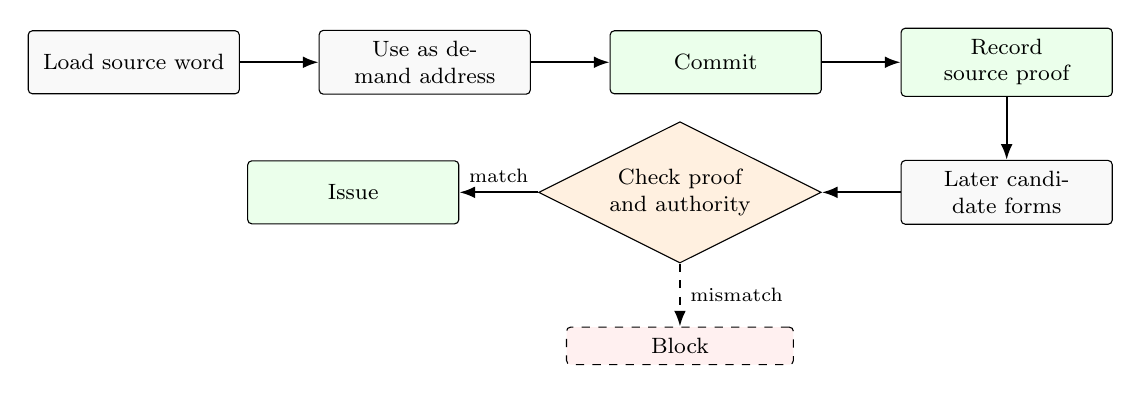
\begin{tikzpicture}[copperpicture]
\node[copperbox] (load) {Load source word};
\node[copperbox, right=of load] (use) {Use as demand address};
\node[copperok, right=of use] (commit) {Commit};
\node[copperok, right=of commit] (record) {Record source proof};
\node[copperbox, below=of record] (candidate) {Later candidate forms};
\node[coppergate, left=of candidate] (check) {Check proof and authority};
\node[copperok, left=of check] (issue) {Issue};
\node[copperblock, below=of check] (block) {Block};
\draw[copperarrow] (load) -- (use);
\draw[copperarrow] (use) -- (commit);
\draw[copperarrow] (commit) -- (record);
\draw[copperarrow] (record) -- (candidate);
\draw[copperarrow] (candidate) -- (check);
\draw[copperarrow] (check) -- node[above, font=\scriptsize] {match} (issue);
\draw[copperclear] (check) -- node[right, font=\scriptsize] {mismatch} (block);
\end{tikzpicture}
\caption{Committed provenance update timeline.}
\label{fig:timeline}
\end{figure}

COPPER has three core rules: proof creation occurs after committed architectural evidence; writes, coherence updates, failed permissions, and context mismatch block or destroy proof; recursive issue does not gain authority merely because a line arrived by prefetch.

\section{Implementation}
The artifact contains a Python model, a trace-driven evaluation harness, SystemVerilog RTL units, C/C++ workload sources, reproduction scripts, and summary parsers. The open-source RTL smoke target is \path{copper_prefetch_unit_open}; larger local Vivado summaries are treated as existing evidence rather than portable rerun proof. The gem5 evidence is validated through retained summaries and provenance files where available \cite{binkert2011gem5}; the open-source full-core hardware harness uses PicoRV32 rather than a production ARM/OoO target \cite{wolf2019picorv32}.

\section{Methodology}
\begin{table}[H]
\centering
\caption{Benchmarks}
\begin{tabularx}{\linewidth}{lYY}
\hline
Class & Examples & Evidence file \\
\hline
Pointer-heavy & linked list, tree, hash, graph, Patricia & workload\_build.csv; independent\_sim\_performance.csv \\
Controls & array, matrix, compute, random access & workload\_build.csv; independent\_sim\_performance.csv \\
Stress & short chains, long chains, mixed, noisy, branchy & workload\_build.csv; independent\_sim\_performance.csv \\
\hline
\end{tabularx}
\end{table}

\begin{table}[H]
\centering
\caption{Configurations And Baselines}
\begin{tabularx}{\linewidth}{lYY}
\hline
Config & Role & Evidence file \\
\hline
no\_prefetch & reference & cycle\_performance.csv \\
next\_line & spatial baseline & cycle\_performance.csv \\
stride & regular-stream baseline & cycle\_performance.csv \\
simple\_pointer\_chase & unsafe content-derived baseline & cycle\_performance.csv \\
copper & committed-provenance policy & cycle\_performance.csv \\
\hline
\end{tabularx}
\end{table}

The normalized CSVs report per-workload rows rather than hiding negative results inside averages. Evidence levels are explicit: \texttt{model} rows come from the executable policy model, \texttt{cycle\_model} rows come from a deterministic memory-system model with hit/miss latency, memory latency, outstanding prefetches, queue drops, lateness, and demand/prefetch traffic accounting. \texttt{core\_integrated} rows add a deterministic core envelope with fetch/issue width, reorder-window pressure, load-queue pressure, branch penalties, and memory-system timing. \texttt{independent\_sim} rows execute the source-built C workload driver for checksums and then use a separate trace/event cache simulator that does not import the cycle-model or core-integrated harness. \texttt{gem5\_full\_system} rows are imported from validated ARM-system summaries only when the compared group has a no-prefetch baseline, a COPPER-family row, matching checksums, zero return codes, and positive tick counts. \texttt{gem5\_statistical\_summary.csv} reports imported-summary confidence intervals where repeated samples exist and marks single-sample rows explicitly. This paper does not claim a clone-local rerun of every raw simulator run. None of these rows claim complete CPU integration.

\section{Evaluation}
\begin{figure}[H]
\centering
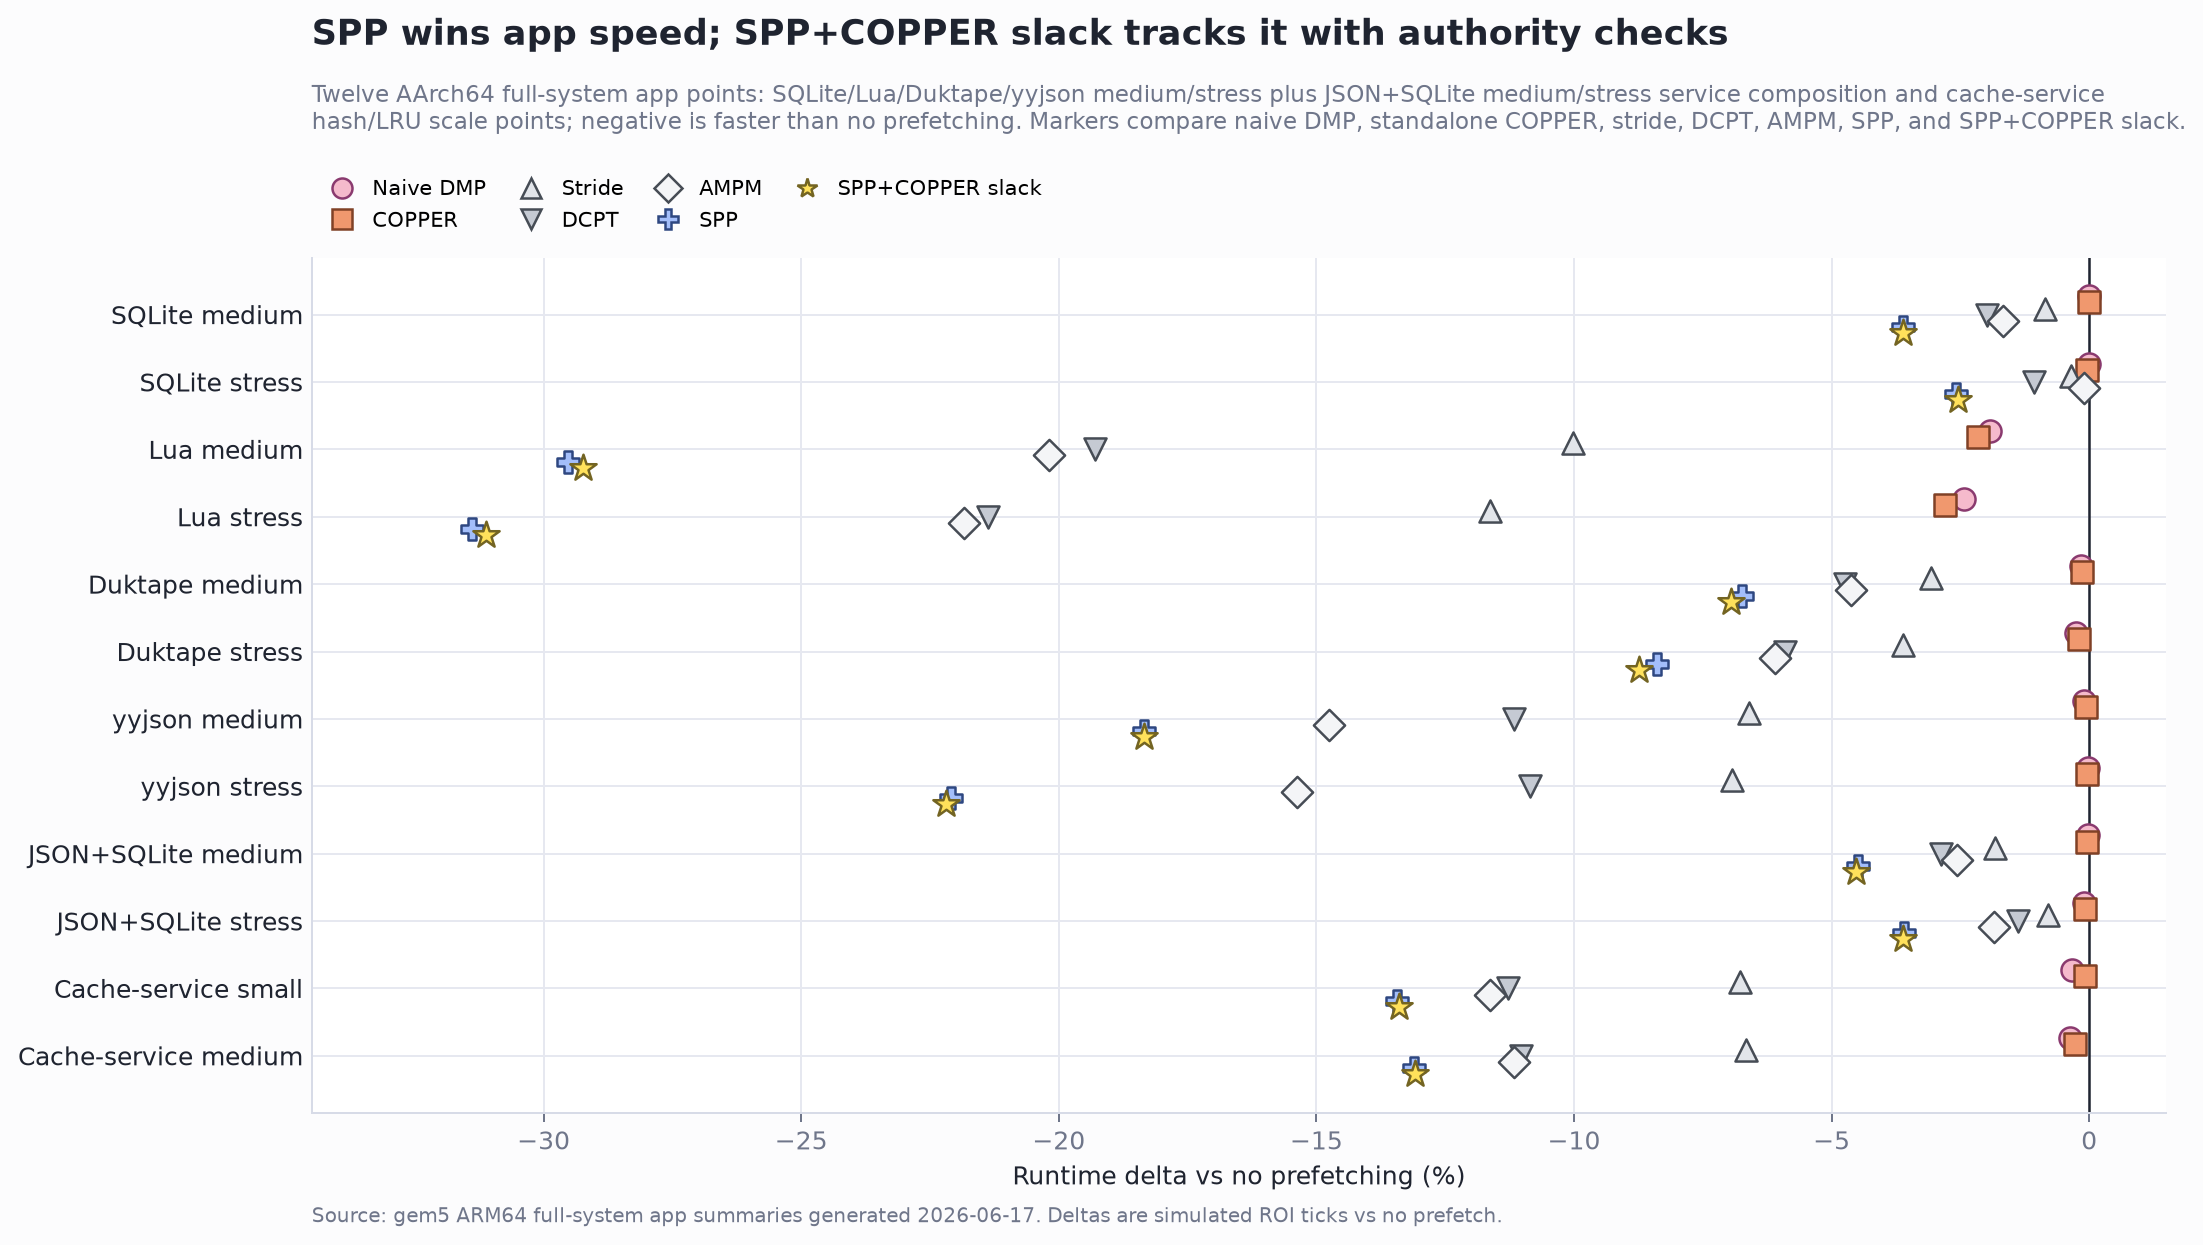
\includegraphics[width=\linewidth]{copper_app_full_baseline_runtime.png}
\caption{Application runtime deltas from the generated AArch64 application figure set. The plot keeps conventional SPP, SPP+COPPER slack, standalone COPPER, and unsafe data-derived baselines visible so authority and speed are discussed separately.}
\label{fig:speedup}
\end{figure}

\begin{figure}[H]
\centering
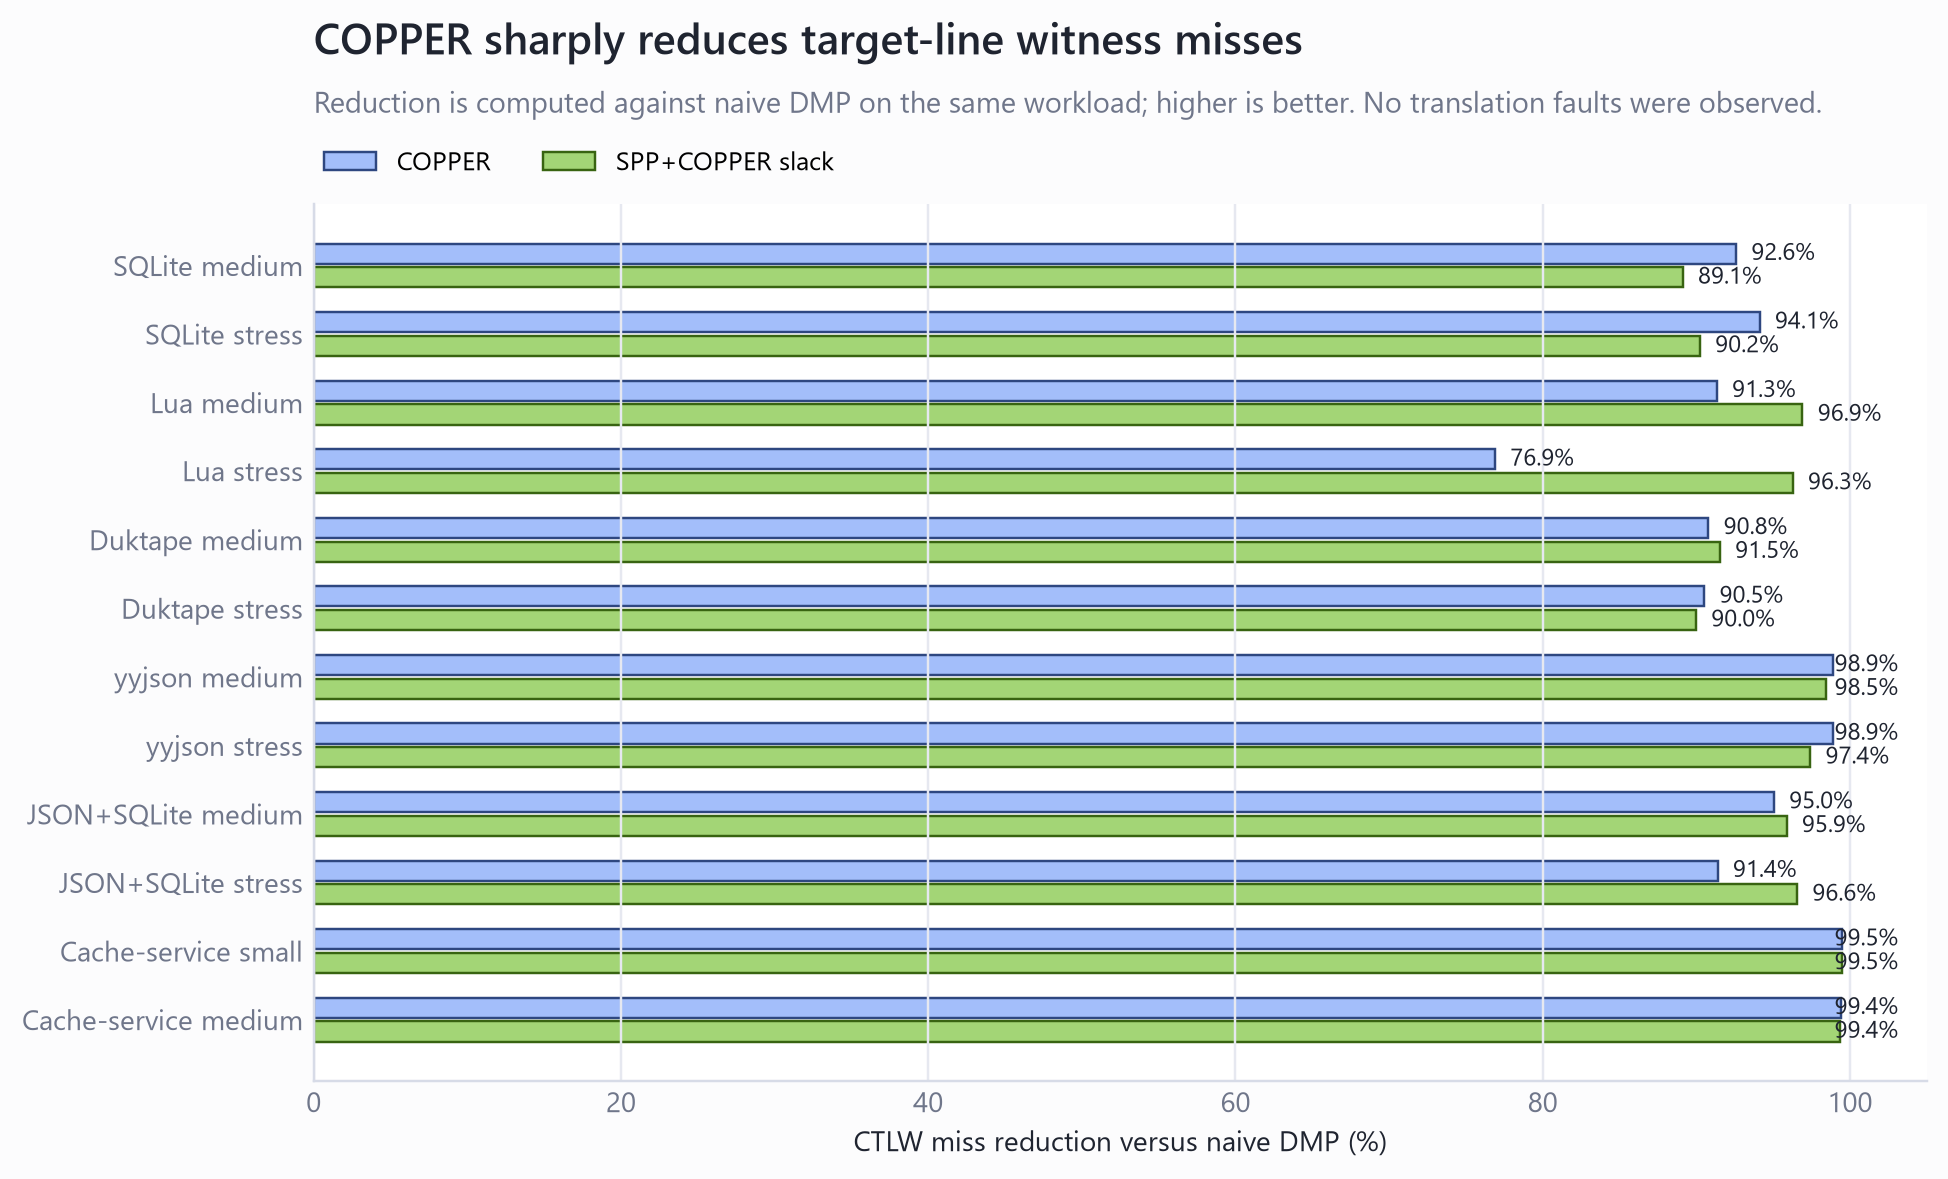
\includegraphics[width=\linewidth]{copper_app_ctlw_reduction.png}
\caption{Target-line witness miss reduction against the unsafe data-derived baseline. This figure supports the authority-safety discussion rather than a universal performance claim.}
\label{fig:prefetch}
\end{figure}

\begin{figure}[H]
\centering
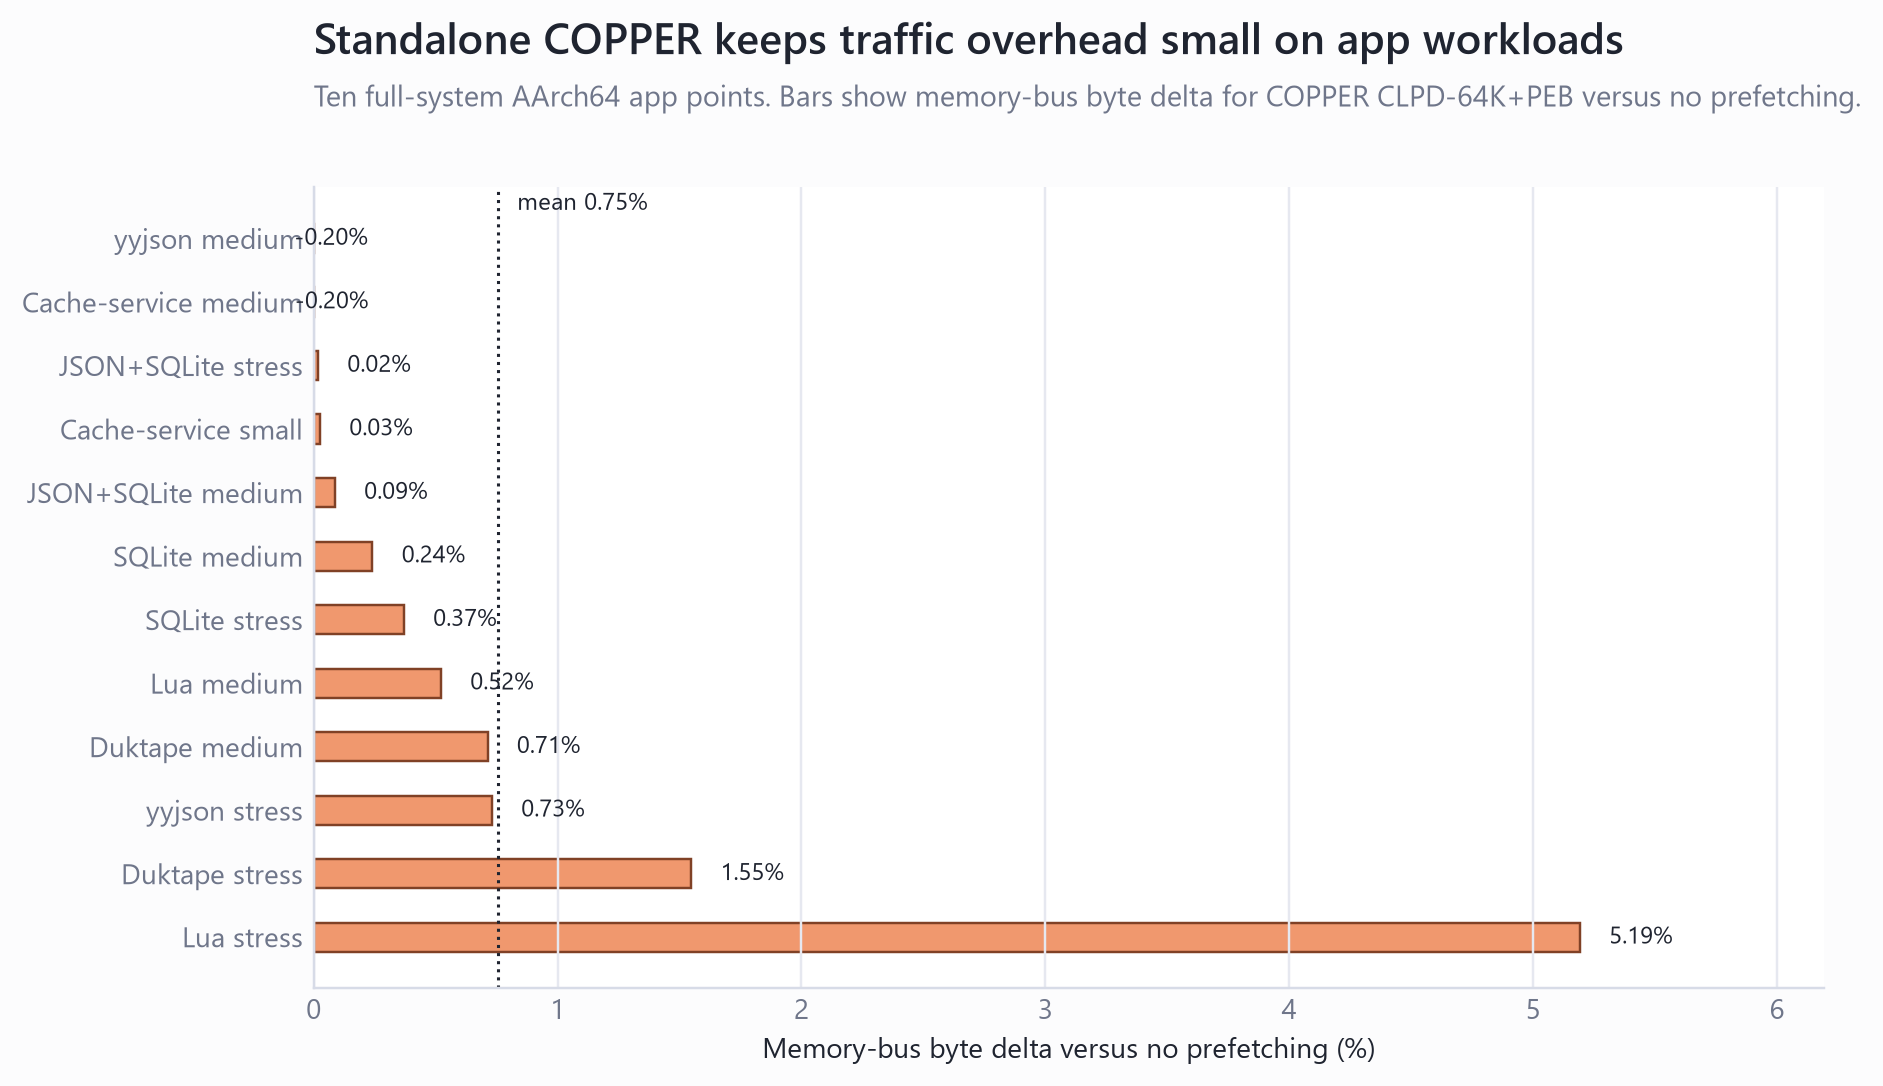
\includegraphics[width=\linewidth]{copper_app_bus_overhead.png}
\caption{Memory-bus byte deltas for standalone COPPER on the generated application workload points. The figure is used only for evidence-level traffic discussion and is not a silicon-power measurement.}
\label{fig:traffic}
\end{figure}

\begin{table}[H]
\centering
\caption{Result Figure Provenance}
\label{tab:figure-provenance}
\begin{tabularx}{\linewidth}{lYY}
\hline
Figure & Source image & Data and producer \\
\hline
\ref{fig:speedup} & \path{copper_app_full_baseline_runtime.png} & \path{copper_prefetch_traffic_overhead_20260616.csv}; \path{plot_copper_app_full_baseline_runtime.py} \\
\ref{fig:prefetch} & \path{copper_app_ctlw_reduction.png} & \path{copper_prefetch_traffic_overhead_20260616.csv}; \path{plot_copper_app_overhead_figures.py} \\
\ref{fig:traffic} & \path{copper_app_bus_overhead.png} & \path{copper_prefetch_traffic_overhead_20260616.csv}; \path{plot_copper_app_overhead_figures.py}; \path{COPPER_APP_FIGURE_INDEX_20260616.md} \\
\hline
\end{tabularx}
\end{table}

Current evidence supports selective, per-workload discussion. Several cycle-model, core-integrated, and independent-sim rows show COPPER behind the best baseline; those regressions remain in the CSVs and block a universal speedup claim.

\section{Ablation And Sensitivity}
\begin{figure}[H]
\centering
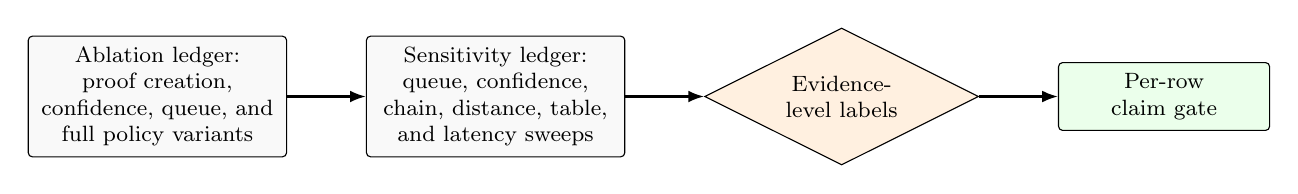
\begin{tikzpicture}[copperpicture]
\node[copperwide] (abl) {Ablation ledger: proof creation, confidence, queue, and full policy variants};
\node[copperwide, right=of abl] (sens) {Sensitivity ledger: queue, confidence, chain, distance, table, and latency sweeps};
\node[coppergate, right=of sens] (label) {Evidence-level labels};
\node[copperok, right=of label] (claim) {Per-row claim gate};
\draw[copperarrow] (abl) -- (sens);
\draw[copperarrow] (sens) -- (label);
\draw[copperarrow] (label) -- (claim);
\end{tikzpicture}
\caption{Ablation and sensitivity evidence flow. The CSV ledgers preserve scope labels so cycle-model counters are not presented as gem5 or hardware counters.}
\label{fig:ablation}
\end{figure}

The cycle-model ablations isolate no provenance, speculative provenance, committed-only proof, confidence, queue filtering, and full COPPER. Queue size, confidence threshold, chain depth, distance, table size, and memory latency are varied in sensitivity rows. These are cycle-model counters and should not be described as gem5 counters.

\section{Hardware Cost}
\begin{table}[H]
\centering
\caption{Hardware Cost}
\begin{tabularx}{\linewidth}{YYY}
\hline
Evidence & Scope & File \\
\hline
CI RTL simulation & open-source unit test & rtl\_simulation.csv \\
Yosys & generic unit resource context & synthesis.csv \\
nextpnr & mapped unit resource context when available & synthesis.csv \\
Overhead & matched unit rows from same flow & synthesis\_overhead.csv \\
Near-core stub & matched generic near-core-stub rows when Yosys runs & fullcore\_synthesis\_overhead.csv \\
PicoRV32 core-wrapper & matched generic accepted core-wrapper rows when Yosys runs & fullcore\_synthesis\_overhead.csv \\
PicoRV32 tiny-SoC full-core & matched full-core rows when Yosys or mapped flows run & fullcore\_synthesis\_overhead.csv; mapped\_ppa.csv \\
Mapped PPA & matched near-core-stub, PicoRV32 core-wrapper, PicoRV32 tiny-SoC full-core, or unit rows only when place-and-route succeeds & mapped\_ppa.csv; mapped\_ppa\_overhead.csv \\
Production-core integration & not claimed & top\_tier\_gate\_status.csv \\
\hline
\end{tabularx}
\end{table}

The artifact supports unit-level hardware plausibility, matched near-core-stub resource-overhead rows, matched PicoRV32 accepted-core-wrapper rows, and matched PicoRV32 tiny-SoC full-core rows when the generated ledgers mark them PASS. The near-core stub is not a full CPU, the accepted wrapper is not full-core, and the PicoRV32 tiny-SoC full-core harness is not a production ARM/OoO integration. Generic Yosys rows do not provide mapped timing, Fmax, ASIC area, or measured power. Mapped timing may be discussed only when \path{mapped_ppa.csv} contains matched PASS rows from nextpnr, Vivado, or OpenROAD.

\section{Energy Proxy}
\begin{table}[H]
\centering
\caption{Energy/Power Evidence}
\begin{tabularx}{\linewidth}{YYY}
\hline
Evidence & Scope & File \\
\hline
Memory traffic proxy & assumption-based, not measured & energy\_proxy.csv \\
ASIC Liberty tool-power index & Nangate45 standard-cell estimate when indexed PASS & asic\_power.csv; power\_report\_index.csv \\
OpenROAD post-route power index & Nangate45 post-route tool estimate with indexed final DEF/SPEF/netlist when PASS & openroad\_postroute\_power.csv; power\_report\_index.csv \\
FPGA tool-power index & Vivado FPGA tool estimate when indexed PASS & power\_report\_index.csv; mapped\_ppa.csv \\
Activity proxy & McPAT proxy when indexed PASS & power\_report\_index.csv; copper\_mcpat\_sensitivity\_20260618.csv \\
Summary & proxy overhead statistics & energy\_summary.csv \\
\hline
\end{tabularx}
\end{table}

Energy rows use explicit assumptions recorded in \path{energy_proxy.csv}. When the power index marks OpenROAD post-route tool estimates as PASS, the row is a Nangate45 OpenROAD-flow-scripts post-route estimate with indexed final DEF/SPEF/netlist artifacts, not silicon measurement or foundry signoff. When ASIC Liberty tool estimates are PASS, the row is a Nangate45 standard-cell Liberty estimate from OpenSTA/OpenROAD, not silicon measurement or post-route signoff with extracted parasitics. When FPGA tool estimates are PASS, the row is Vivado report power for the mapped FPGA target, not silicon or ASIC signoff. Activity-proxy PASS rows are fixed-architecture McPAT sensitivity runs driven by measured gem5 ROI counters. This supports evidence-level tool-power and proxy/model energy discussion, not foundry-signoff or silicon power-efficiency claims.

\section{Limitations}
\begin{table}[H]
\centering
\caption{Limitations}
\begin{tabularx}{\linewidth}{YY}
\hline
Limitation & Consequence \\
\hline
Gem5 rows are validated imported ARM-system summaries & Gem5 validation applies to imported PASS rows \\
Independent simulator is trace/event level & It is not a replacement for a broad gem5 campaign \\
PicoRV32 tiny-SoC is the open-source full-core target & Production ARM/OoO claims remain blocked \\
Power is tool-estimate/model based & Signoff and silicon power-efficiency claims remain blocked \\
External gem5 and Vivado setup & Large external-tool reruns are not clone-local \\
\hline
\end{tabularx}
\end{table}

\section{Artifact Evidence Gates}
\begin{table}[H]
\centering
\caption{Artifact And Evidence Gates}
\begin{tabularx}{\linewidth}{YYY}
\hline
Gate class & Status source & Interpretation \\
\hline
CI RTL evidence & rtl\_simulation.csv & GitHub Actions unit simulation \\
Cycle-model evidence & cycle\_performance.csv & deterministic memory-system timing model \\
Core-integrated evidence & core\_integrated\_performance.csv & deterministic core-envelope model \\
Independent simulator & independent\_sim\_performance.csv & source-backed trace/event simulator \\
Gem5 validated summaries & gem5\_validation.csv; gem5\_performance.csv; gem5\_statistical\_summary.csv & imported ARM-system rows and imported-summary statistics when PASS \\
Hardware cost & synthesis\_overhead.csv; fullcore\_synthesis\_overhead.csv; mapped\_ppa.csv & matched unit, near-core-stub, PicoRV32 core-wrapper, or PicoRV32 tiny-SoC full-core resources, plus mapped timing only when PASS \\
Energy proxy & energy\_proxy.csv; openroad\_postroute\_power.csv; asic\_power.csv; power\_report\_index.csv & assumption-based proxy plus OpenROAD post-route, ASIC Liberty, or FPGA tool estimates when indexed PASS \\
Package & artifact\_manifest.csv & included and excluded files \\
\hline
\end{tabularx}
\end{table}

\section{Conclusion}
COPPER is best framed as a committed-provenance authority mechanism for data-derived prefetch issue. The artifact supports that claim with a CI-proven open-source path, deterministic cycle-model and core-integrated evidence, source-backed independent-simulator rows, validated imported gem5 ARM-system rows with imported-summary statistics, matched unit-level, near-core-stub, PicoRV32 accepted-core-wrapper, and PicoRV32 tiny-SoC full-core FPGA PPA paths, FPGA tool-estimated power where indexed PASS, proxy energy rows, a claim ledger, audits, and a package manifest. The honest next step for broader production/silicon claims is a final raw-rerunnable gem5 or comparable external core validation matrix plus signoff-calibrated or silicon-measured power evidence without changing the evidence-bounded claims in this artifact.

\bibliographystyle{plain}
\bibliography{references}
\end{document}
